\documentclass{article}
\usepackage[utf8]{inputenc}
\usepackage[T1]{fontenc}
\usepackage{graphicx}
\usepackage{amsmath, amssymb}
\usepackage{xcolor}
\usepackage{tikz}
\usepackage{enumitem}
\usepackage{lipsum}
\usetikzlibrary{fit}
\usepackage{hyperref} 
\usepackage{subfig}
\usepackage{xcolor}
\usepackage{colortbl}
\usepackage{pgfplots}
\pgfplotsset{compat=1.17}
% Define colors
\definecolor{lessoncolor}{RGB}{74, 144, 226}
\definecolor{examplecolor}{RGB}{92, 184, 92}
\definecolor{notecolor}{RGB}{255, 179, 102}

% Define a command for colorful sections
\newcommand{\colorsection}[1]{\section*{\textcolor{lessoncolor}{#1}}}

% Set up TikZ for graphing
\usetikzlibrary{positioning, arrows.meta, shapes.geometric}
\usetikzlibrary{decorations.pathreplacing}

% Document
\begin{document}

\begin{titlepage}
    \centering
    \vspace*{2cm}
    {\LARGE \textcolor{lessoncolor}{Advanced Functions}}\par
    \vspace{1cm}
    {\large Kensukeken}\par
    \vspace{2cm}
    {\large February 22, 2024}\par
    \vspace{3cm}
\end{titlepage}
\tableofcontents
\newpage


\section*{Review}
\subsection{Exponent Laws}
 
\subsubsection*{Product Law}
When multiplying two terms with the same base, add the exponents.
\[ a^m \cdot a^n = a^{m + n} \]

\subsubsection*{Quotient Law}
When dividing two terms with the same base, subtract the exponents.
\[ \frac{a^m}{a^n} = a^{m - n} \]

\subsubsection*{Power Law}
When raising a power to another power, multiply the exponents.
\[ (a^m)^n = a^{mn} \]

\subsubsection*{Zero Exponent Law}
Any nonzero number raised to the power of zero is equal to 1.
\[ a^0 = 1 \]

\subsubsection*{Negative Exponent Law}
\[ a^{-n} = \frac{1}{a^n} \]
\subsubsection*{FOIL}
 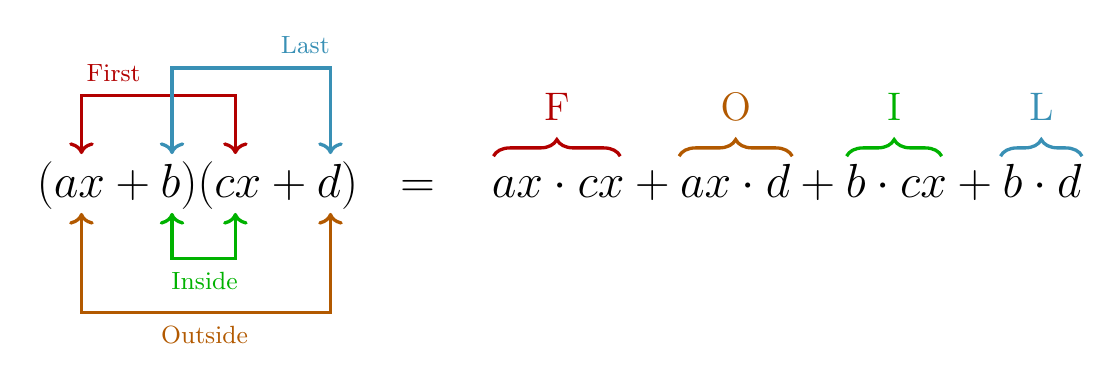
\begin{tikzpicture}[scale=1.15]
 \node[anchor=west] at (0.25,2.0) {\LARGE$(ax+b)(cx+d) \ \ = \quad ax\cdot cx  + ax\cdot d + b \cdot cx  + b\cdot d$};

 \draw[very thick, red!70!black,<->] (0.85,2.35)--(0.85,3.0)--(2.55,3.0)--(2.55,2.35);
   \node[right] at (0.8,3.25) {\color{red!70!black} \small First};
 \draw[very thick, cyan!70!black,<->] (1.85,2.35)--(1.85,3.3)--(3.6,3.3)--(3.6,2.35);
   \node[left] at (3.7,3.55) {\color{cyan!70!black} \small Last};
 \draw[very thick, green!70!black,<->] (1.85,1.7)--(1.85,1.2)--(2.55,1.2)--(2.55,1.7);
   \node[ ] at (2.21,0.95) {\color{green!70!black} \small Inside};
 \draw[very thick, orange!70!black,<->] (0.85,1.7)--(0.85,0.6)--(3.6,0.6)--(3.6,1.7);
   \node[ ] at (2.21,0.35) {\color{orange!70!black} \small Outside};


 %braces
 \draw [very thick,decorate, red!70!black, decoration={brace, amplitude=6pt, raise=2.5pt}] (5.4,2.25)--(6.8,2.25) node [ midway, above=0.4cm] {\Large \color{red!70!black} F};
 \draw [very thick,decorate, orange!70!black, decoration={brace, amplitude=6pt, raise=2.5pt}] (7.45,2.25)--(8.7,2.25) node [ midway, above=0.4cm] {\Large \color{orange!70!black} O};
 \draw [very thick,decorate, green!70!black, decoration={brace, amplitude=6pt, raise=2.5pt}] (9.3,2.25)--(10.35,2.25) node [ midway, above=0.4cm] {\Large \color{green!70!black} I};
 \draw [very thick,decorate, cyan!70!black, decoration={brace, amplitude=6pt, raise=2.5pt}] (11,2.25)--(11.9,2.25) node [ midway, above=0.4cm] {\Large \color{cyan!70!black} L};
 \end{tikzpicture}
\newpage
\subsection{Common Number Sets}

\subsubsection*{Natural Numbers ($\mathbb{N}$)}
The set of natural numbers is denoted by $\mathbb{N}$ and includes all positive integers from 1 onwards. 
\[ \mathbb{N} = \{1, 2, 3, 4, \ldots\} \]

\subsubsection*{Integers ($\mathbb{Z}$)}
The set of integers is denoted by $\mathbb{Z}$. It includes all whole numbers, both positive and negative, including zero.
\[ \mathbb{Z} = \{\ldots, -3, -2, -1, 0, 1, 2, 3, \ldots\} \]

\subsubsection*{Rational Numbers ($\mathbb{Q}$)}
The set of rational numbers is denoted by $\mathbb{Q}$. It includes all numbers that can be expressed as a fraction of two integers, where the denominator is not zero.
\[ \mathbb{Q} = \left\{\frac{a}{b} \mid a,b \in \mathbb{Z}, b \neq 0\right\} \]

\subsubsection*{Real Numbers ($\mathbb{R}$)}
The set of real numbers is denoted by $\mathbb{R}$. It includes all rational and irrational numbers, forming the continuum on the number line.

\subsubsection*{Complex Numbers ($\mathbb{C}$)}
The set of complex numbers is denoted by $\mathbb{C}$. It includes all numbers of the form $a + bi$, where $a$ and $b$ are real numbers and $i$ is the imaginary unit.

\begin{figure}[ht]
    \centering
    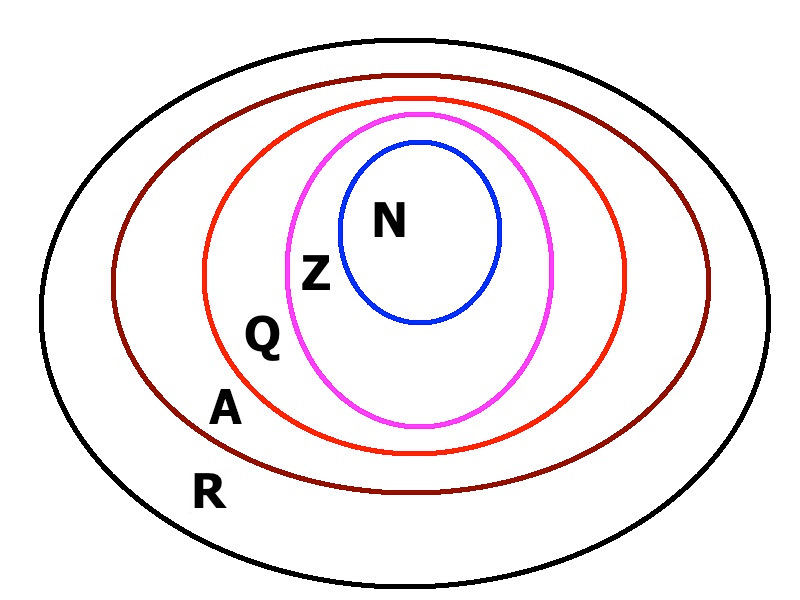
\includegraphics[width=0.35\textwidth]{imgs/number-sets-nzqar.jpg}
    \end{figure}

\newpage    
\section{Unit 1}
\subsection{Power Functions}

\begin{minipage}[t]{\textwidth}
Linear and Quadratic functions are the two most encountered polynomial functions. Polynomials are defined as follows...

A polynomial expression is an expression of the form
\[
a_n x^n + a_{n-1} x^{n-1} + a_{n-1} x^{n-2} + \ldots + a_3 x^3 + a_2 x^2 + a_1 x + a_0,
\]
where
\begin{itemize}
    \item \( n \) is a whole number
    \item \( x \) is a variable
    \item the coefficients \( a_0, a_1, \ldots, a_n \) are real numbers
    \item the degree of the function is \( n \), the exponent of the greatest power of \( x \)
    \item \( a_n \), the coefficient of the greatest power of \( x \), is the leading coefficient
    \item \( a_0 \), the term without a variable, is the constant term
\end{itemize}

A polynomial function has the form
\[
f(x) = a_n x^n + a_{n-1} x^{n-1} + a_{n-2} x^{n-2} + \ldots + a_5 x^3 + a_2 x^2 + a_1 x + a_0
\]

Power functions, the simplest polynomial functions, have one term and transform into a general polynomial function when transformed.
\end{minipage}

\vspace{0.5cm}

\begin{center}
\begin{minipage}[t]{0.8\textwidth}
\centering
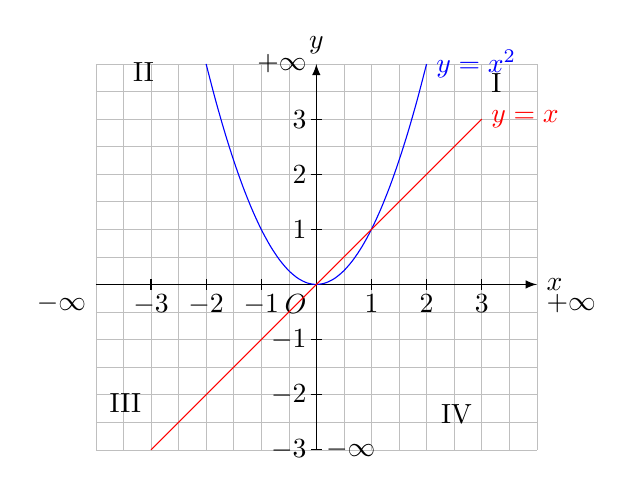
\begin{tikzpicture}[>=latex, scale=0.7]
    % Grid
    \draw[xstep=0.5,ystep=0.5,gray!50,very thin] (-4,-3) grid (4,4);
    % Axes
    \draw[->] (-4,0) -- (4,0) node[right] {$x$};
    \draw[->] (0,-3) -- (0,4) node[above] {$y$};
    % Label x and y axes
    \foreach \x in {-3,-2,-1,1,2,3}
        \draw (\x,-0.1) -- (\x,0.1) node[below=2pt] {$\x$};
    \foreach \y in {-3,-2,-1,1,2,3}
        \draw (-0.1,\y) -- (0.1,\y) node[left=2pt] {$\y$};
    % Label infinity
    \node[below right] at (4,0) {$+\infty$};
    \node[left] at (0,4) {$+\infty$};
    \node[below left] at (-4,0) {$-\infty$};
    \node[right] at (0,-3) {$-\infty$};
    % Label quarters
    \node[below left] at (0,0) {$O$};
    \node[below right] at (3,4) {I};
    \node[above right] at (-3.5,3.5) {II};
    \node[above left] at (-3,-2.5) {III};
    \node[below left] at (3,-2) {IV};
    % Plot y=x^2
    \draw[domain=-2:2,smooth,variable=\x,blue] plot ({\x},{\x*\x}) node[right] {$y=x^2$};
    % Plot y=x
    \draw[domain=-3:3,smooth,variable=\x,red] plot ({\x},{\x}) node[right] {$y=x$};
\end{tikzpicture}
\end{minipage}\\


\end{center}

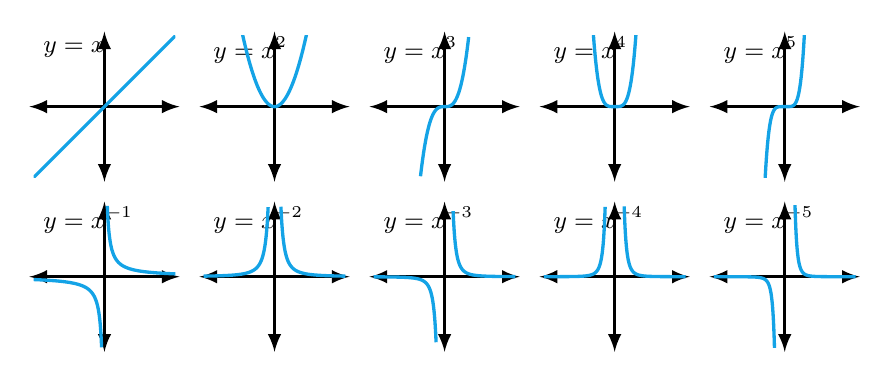
\begin{tikzpicture}[scale=0.3] 

\foreach \e/\d [count=\i] in {1/5,2/2.3,3/1.7,4/1.5,5/1.5,-1/0.2,-2/0.45,-3/0.6,-4/0.67,-5/0.7} {
  \ifnum\e < 0
    \pgfmathsetmacro\row{0};
  \else 
    \pgfmathsetmacro\row{1};
  \fi

  \begin{scope}[scale=0.6, xshift=abs(\e)*12 cm, yshift=\row*12 cm] 
    \ifnum\e = 1
      \node[right] at (-5,4) {\small $y=x$};
    \else 
      \node[right] at (-5,4) {\small $y=x^{\e}$};
    \fi

    \draw[latex-latex, very thick] (-5.3,0)--(5.3,0);
    \draw[latex-latex, very thick] (0,-5.3)--(0,5.3);

    \begin{scope}
      \clip(-5,-5) rectangle (5,5);
      \ifnum\e > 0
        \draw[domain=-\d:\d, smooth, variable=\x, Cerulean, samples=120, very thick] plot ({\x},{(\x)^(\e) });
      \else 
        \draw[domain=-5:-\d, smooth, variable=\x, Cerulean, samples=120, very thick] plot ({\x},{(\x)^(\e) });
        \draw[domain=\d:5, smooth, variable=\x, Cerulean, samples=120, very thick] plot ({\x},{(\x)^(\e) });
      \fi 
    \end{scope}
  \end{scope}
}
 
\end{tikzpicture} \\
To explore Polynomial functions along with their powers, functions, special names, graphs, domains, ranges, and end behaviors as well as leading terms, refer to the \href{run:./Unit\%201\%20-\%20Polynomial\%20Functions/Polynomial.tex}{Polynomial.tex} file or \href{https://math.libretexts.org/Bookshelves/Precalculus/Precalculus_1e_(OpenStax)/03%3A_Polynomial_and_Rational_Functions/3.03%3A_Power_Functions_and_Polynomial_Functions}{Power Functions and Polynomial Functions}.

\section*{Understanding Function Properties}

\subsection*{Even and Odd Degree Functions}

\textbf{Even Degree Functions:} Graphs that curve from quadrant 3 to quadrant 1. The higher the exponent the closer the curve gets to the y-axis.\\
\textbf{Odd Degree Functions:} Graphs that make a U-shape. The higher the exponent the U shape gets closer to the y-axis. 

\begin{center}
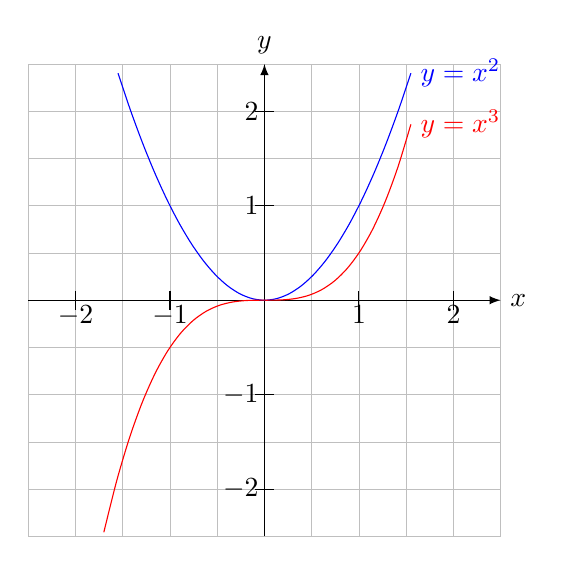
\begin{tikzpicture}[>=latex, scale=1.2]
  % Grid
  \draw[xstep=0.5,ystep=0.5,gray!50,very thin] (-2.5,-2.5) grid (2.5,2.5);
  % Axes
  \draw[->] (-2.5,0) -- (2.5,0) node[right] {$x$};
  \draw[->] (0,-2.5) -- (0,2.5) node[above] {$y$};
  % Labels
  \foreach \x in {-2,-1,1,2}
      \draw (\x,-0.1) -- (\x,0.1) node[below=2pt] {$\x$};
  \foreach \y in {-2,-1,1,2}
      \draw (-0.1,\y) -- (0.1,\y) node[left=2pt] {$\y$};
  % Even function
  \draw[domain=-1.55:1.55,smooth,variable=\x,blue] plot ({\x},{\x*\x}) node[right] {$y=x^2$};
  % Odd function
  \draw[domain=-1.70:1.55,smooth,variable=\x,red] plot ({\x},{0.5*\x*\x*\x}) node[right] {$y=x^3$};
\end{tikzpicture}
\end{center}
\newpage 
\subsection*{Understanding End Behavior}

\textbf{End Behavior:} The end behaviour of a function is the behaviour of the y-values as x increases  (that is, as x approaches positive infinity, $x\to \infty$) and as x decreases (that is, as x approaches negative infinity, $x \to -\infty$)\\

\begin{center}
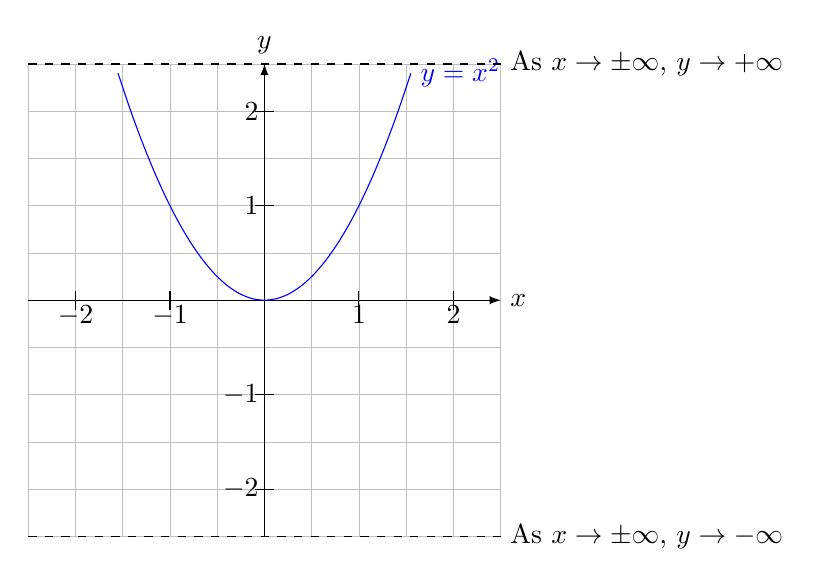
\begin{tikzpicture}[>=latex, scale=1.2]
  % Grid
  \draw[xstep=0.5,ystep=0.5,gray!50,very thin] (-2.5,-2.5) grid (2.5,2.5);
  % Axes
  \draw[->] (-2.5,0) -- (2.5,0) node[right] {$x$};
  \draw[->] (0,-2.5) -- (0,2.5) node[above] {$y$};
  % Labels
  \foreach \x in {-2,-1,1,2}
      \draw (\x,-0.1) -- (\x,0.1) node[below=2pt] {$\x$};
  \foreach \y in {-2,-1,1,2}
      \draw (-0.1,\y) -- (0.1,\y) node[left=2pt] {$\y$};
  % Even function
  \draw[domain=-1.55:1.55,smooth,variable=\x,blue] plot ({\x},{\x*\x}) node[right] {$y=x^2$};
  % End behaviors
  \draw[dashed] (-2.5,2.5) -- (2.5,2.5) node[right] {As $x \rightarrow \pm\infty$, $y \rightarrow +\infty$};
  \draw[dashed] (-2.5,-2.5) -- (2.5,-2.5) node[right] {As $x \rightarrow \pm\infty$, $y \rightarrow -\infty$};
\end{tikzpicture}
\end{center}

\subsection*{Properties of Power Functions}

\textbf{Domain and Range:} 
For power functions, the domain is all real numbers ($x \in \mathbb{R}$), and the range depends on whether the function is even or odd.\\
\textbf{Symmetry:} Power functions exhibit symmetry properties based on whether they are even or odd functions. 

\subsubsection{Deriving Polynomial Functions from Data:}

\begin{table}[h]
    \centering
    \begin{tabular}{|c|c|c|}
    \hline
        \rowcolor[HTML]{EFEFEF}
        $x$ & $y$ & $\Delta f(x)$ \\
        \hline
        1 & 1 & $2-1$\\
        \hline
        2 & 2 & \\
        \hline
        3 & 3 & \\
        \hline
        4 & 4 & $\vdots$ \\
        \hline
        $\vdots$ & $\vdots$ & $\vdots$\\
        \hline
        $m-1$ & $m-1$ & $m-(m-1)$\\
        \hline
        $m$ & $m$ & $m+1-m$\\
        \hline
        $m+1$ & $m+1$ & \\
        \hline
    \end{tabular}
    \caption*{The set of first differences for a linear function remains constant.}
\end{table}

\newpage
\section*{Union and Intersection}
If $A=\{1,3,5,7,9\}$ and $B=\{2,3,5,7$,$\} , what are A \cup B$ and $A \cap B$ ?

We have
$$
\begin{aligned}
& A \cup B=\{1,2,3,5,7,9\} \\
& A \cap B=\{3,5,7\} \cdot 
\end{aligned}
$$


\def\firstcircle{(0,0) circle (1cm)}
\def\secondcircle{(0:1.5cm) circle (1cm)}

\colorlet{circle edge}{blue!50}
\colorlet{circle area}{blue!20}

\tikzset{
    filled/.style = {fill=circle area, draw=circle edge, thick},
    outline/.style = {draw=circle edge, thick},
    F/.style = {draw, inner sep=7mm, fit=(current bounding box),
                node contents={}}
}



\begin{center}
\end{center}

\begin{figure}[h]
    \centering
    \begin{minipage}[t]{0.45\linewidth} 
        \centering   
        \begin{tikzpicture}
            \draw[filled] \firstcircle node {$A$}
                          \secondcircle node {$B$};
            \node (a) [F];                 
            \node[below left] at (a.north east) {$A \cup B$};
        \end{tikzpicture}
        \caption{Presentation of sets union by Venn diagram}
        \label{fig:ven-1a}
    \end{minipage}
    \hfil
    \begin{minipage}[t]{0.45\linewidth}
        \centering
        \begin{tikzpicture}
            \begin{scope}
                \clip \firstcircle;
                \fill[filled] \secondcircle;
            \end{scope}
            \draw[outline] \firstcircle node {$A$};
            \draw[outline] \secondcircle node {$B$};
            \node (a) [F];
            \node[below left] at (a.north east) {$A \cap B$};
        \end{tikzpicture}
        \caption{Presentation of sets intersection by Venn diagram}
        \label{fig:ven-1b}
    \end{minipage}% end of subfloat
\end{figure}


Feel free to learn more in \href{https://brilliant.org/wiki/sets-union-and-intersection-easy/#:~:text=The%20union%20of%202%20sets,the%20symbol%20is%20%E2%88%AAnion.}{Union and intersections}

\subsection{Characteristics of Polynomial Function}

A general note: Terminology of polynomial functions:\\
\begin{figure}[h]
    \centering
    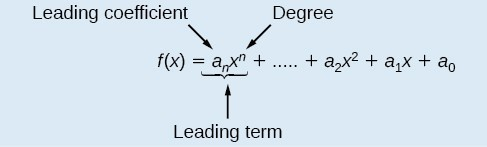
\includegraphics[width=0.6\textwidth]{imgs/polynomial.jpg}
\end{figure}\\
Finite Differences: The nth differences for a polynomial of degree n will all
be the same, and this common difference will be equal to the product of n!
and the leading coefficient $(a_n)$.
\begin{align*}
\text{Common Difference} &= a_nn! (a_n \times n!)\\
&= a_n[n \times (n-1) \times (n-2) \times \cdots \times 3 \times 2 \times 1]
\end{align*}
where, 
\begin{itemize}
    \item \(a_n\) represents the \(n\)th term of the arithmetic sequence.
    \item \(n!\) represents the factorial of \(n\), which is the product of all positive integers up to \(n\). For example, \(5! = 5 \times 4 \times 3 \times 2 \times 1\).
\end{itemize}

\subsubsection*{Example:}The finite differences are taken for a polynomial function, and the 6th differences are found to all be -2880. What was the
leading coefficient of the polynomial function.
Given:
\[
\text{Common Difference} = -2880 = a \times 6!
\]

We are trying to find the value of \(a\). So, let's solve for \(a\):

\[a = \frac{-2880}{6!} = \frac{-2880}{720} = -4\]

So, the value of \(a\) is indeed \(-4\).
\subsubsection{Anatomy of a Polynomial Function:}
\begin{figure}[ht]
    \centering
    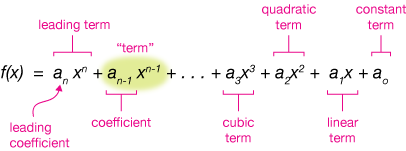
\includegraphics[width=0.6\textwidth]{imgs/anatomyofapolynomialfunction.png}
\end{figure}


To learn more about the characteristics of polynomial functions, you can visit the following link: \href{https://mathematicalmysteries.org/characteristics-of-polynomials/}{Characteristics of Polynomial Function}.

\subsubsection{Local Minimum and Maximum Points}
Let's look at the graph of the polynomial function defined by $x^3+x^2$.

\begin{minipage}{0.6\linewidth}
\centering
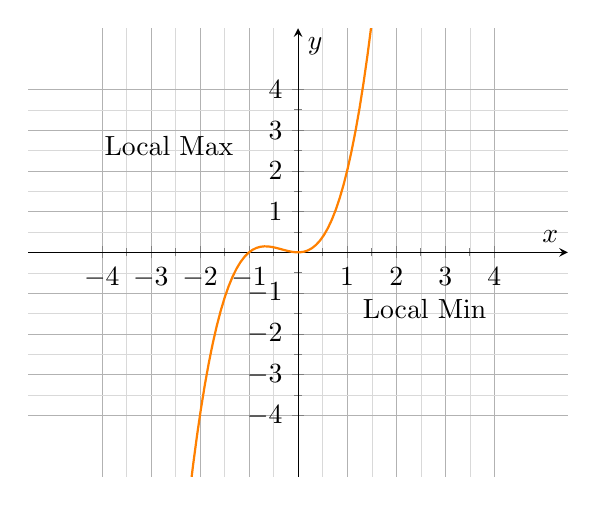
\begin{tikzpicture}
\begin{axis}[
    xlabel=$x$,
    ylabel=$y$,
    axis lines=middle,
    xmin=-5,
    xmax=5,
    ymin=-5,
    ymax=5,
    xtick={-4,...,4},
    ytick={-4,...,4},
    grid=both,
    grid style={line width=.1pt, draw=gray!30},
    major grid style={line width=.2pt,draw=gray!60},
    minor tick num=1,
    enlargelimits={abs=0.5},
]
% Plot the function
\addplot[domain=-4:4, samples=100, thick, orange] {x^3 + x^2};

% Local minimum and maximum points
\node[circle, inner sep=2pt,label={above right: Local Min}] at (axis cs:1,-2) {};
\node[circle,inner sep=2pt,label={above left:Local Max}] at (axis cs:-1,2) {};
\end{axis}
\end{tikzpicture}
\end{minipage}%
\begin{minipage}{0.4\linewidth}
Looks more $f(x)=x^3$ than $f(x)=x^2$, but there is a small change we now have "bumps" on the graph.
\end{minipage}
In general, polynomial function graphs consist of a smooth curve with a series of hills and valleys. The hills and valleys are called turning points. Each \textbf{turning point} corresponds to a \textbf{local maximum} or \textbf{local minimum point}. 
\newpage 
\textbf{Finite Differences:}{ (used to find leading terms and determine degree from a table of values)}
\subsubsection*{Example 1:} 
Recall for linear functions $f(x) = 3x + 2$ we could make a table of values 

\[
\begin{array}{|c|c|c|}
\hline
x & f(x) & \text{First Difference} \\
\hline
0 & 2 & \\
1 & 5 & 3 \\
2 & 8 & 3 \\
3 & 11 & 3 \\
4 & 14 & 3 \\
5 & 17 & 3 \\
\hline
\end{array}
\]
First Difference is constant, so degree is equal to 1 and leading coefficient is 3 
\subsubsection*{Example 2:}

\[
\begin{array}{|c|c|c|c|}
\hline
x & y & \text{1st Difference} & \text{2nd Difference} \\
\hline
0 & 1 & & \\
1 & 6 & 5 & \\
2 & 17 & 11 & 6 \\
3 & 34 & 17 & 6 \\
4 & 57 & 23 & 6 \\
5 & 86 & 29 & 6 \\
\hline
\end{array}
\]
Second Difference is constant, so degree is equal to 2 but the leading coefficient is not 6 it should be 3. So how do we account for this?
For a polynomial of degree \( n \), where \( n \) is a positive integer, the \( n \)th differences:
\begin{itemize}
    \item are constant (equal)
    \item have the same sign as the leading coefficient
    \item are equal to \( a(n!) \), where \( a \) is the leading coefficient
\end{itemize}

Factorial (!) means: \( n! = n(n - 1)(n - 2)(n - 3) \dotsm (2)(1) \)

For example, \( 5! = 5 \times 4 \times 3 \times 2 \times 1 = 120 \).

So for our example above, the second difference is constant, so the degree is equal to 2, but the leading coefficient is \( a(n!) \):

\[ 6 = a(2!) \text{ because } n = 2 \]
\[ 6 = a(2)(1) \]
\[ 6 = 2a \]
\[ 3 = a \]

\subsubsection{Key Features of Polynomial Functions with Odd Degree}

\subsubsection*{Description}

\begin{itemize}
    \item Odd-degree polynomials have at least one zero, up to a maximum of \( n \) x-intercepts, where \( n \) is the degree of the function.
    \item The domain is \( x \in \mathbb{R} \) and the range is \( y \in \mathbb{R} \).
    \item They have no absolute maximum point and no absolute minimum point.
    \item They may have point symmetry.
\end{itemize}

\subsubsection*{Graphical Representation}

\begin{center}
\begin{tikzpicture}[scale=0.7]
% Axes
\draw[-{Stealth}] (-5,0) -- (5,0) node[below] {\( x \)};
\draw[-{Stealth}] (0,-5) -- (0,5) node[left] {\( y \)};
% Function
\draw[domain=-1:1,smooth,variable=\x,red] plot ({\x},{\x^3-\x});
% Annotations
\draw[dashed] (1,0) node[below] {\( 1 \)} -- (1,0 |- 0,1) node[left] {\( f(1) \)};
\draw[dashed] (-1,0) node[below] {\( -1 \)} -- (-1,0 |- 0,-1) node[right] {\( f(-1) \)};
\end{tikzpicture}
\end{center}

\subsubsection*{Positive Leading Coefficient}

\begin{itemize}
    \item Graph extends from quadrant 3 to quadrant 1.
    \item Alternatively, as \( x \to -\infty \), \( y \to -\infty \) and as \( x \to \infty \), \( y \to \infty \).
\end{itemize}

\subsubsection*{Negative Leading Coefficient}

\begin{itemize}
    \item Graph extends from quadrant 2 to quadrant 4.
    \item Alternatively, as \( x \to -\infty \), \( y \to \infty \) and as \( x \to \infty \), \( y \to -\infty \).
\end{itemize}




\subsubsection{Key Features of Polynomial Functions with Even Degree}

\subsubsection*{Description}

\begin{itemize}
    \item Even-degree polynomials may have no zeros, up to a maximum of \( n \) x-intercepts, where \( n \) is the degree of the function.
    \item The domain is \( \{x \in \mathbb{R}\} \).
    \item They may have line symmetry.
\end{itemize}

\subsubsection*{Graphical Representation}

\begin{center}
\begin{tikzpicture}[scale=0.44]
% Axes
\draw[-{Stealth}] (-5,0) -- (5,0) node[below] {\( x \)};
\draw[-{Stealth}] (0,-5) -- (0,5) node[left] {\( y \)};
% Function
\draw[domain=-2:2,smooth,variable=\x,blue] plot ({\x},{\x^2-2});
% Annotations
\draw[dashed] (1,0) node[below] {\( 1 \)} -- (1,0 |- 0,1) node[left] {\( f(1) \)};
\draw[dashed] (-1,0) node[below] {\( -1 \)} -- (-1,0 |- 0,1) node[left] {\( f(-1) \)};
\end{tikzpicture}
\end{center}

\subsubsection*{Positive Leading Coefficient}

\begin{itemize}
    \item Graph extends from quadrant 2 to quadrant 1.
    \item Alternatively, as \( x \to -\infty \), \( y \to \infty \) and as \( x \to \infty \), \( y \to \infty \).
    \item The range is \( \{y \in \mathbb{R} | y \geq a\} \), where \( a \) is the absolute minimum value of the function.
    \item It will have at least one minimum point.
    \item It will have an absolute minimum point.
\end{itemize}

\subsubsection*{Negative Leading Coefficient}

\begin{itemize}
    \item Graph extends from quadrant 3 to quadrant 4.
    \item Alternatively, as \( x \to -\infty \), \( y \to -\infty \) and as \( x \to \infty \), \( y \to -\infty \).
    \item The range is \( \{y \in \mathbb{R} | y \leq a\} \), where \( a \) is the absolute maximum value of the function.
    \item It will have at least one maximum point.
    \item It will have an absolute maximum point.
\end{itemize}


\subsection{Graphs of Polynomial Functions}
\begin{itemize}
    \item The function must be in \textcolor{red}{factored} form to find the x-intercepts.
    \item Plot the x-intercepts, and the y-intercept(get h y-intercept by subbing \textcolor{red}{0} in for x)
    \item Use an \textcolor{red}{interval} test to determine the sign of the polynomial in the intervals divided by the x-intercepts.
    \item The function $f(x)=(x-3)(x-1)(x+2)^2(x+5)^3$ is of degree 7. It has \textcolor{red}{4} intercepts. The zero from the factor $(x+2)^2$ is repeated and so is said to have \textcolor{red}{order} of 2. The zero from the factor $(x+5)^3$ is repeated and so is said to have order $3$.
    \item The function will pass through the axis at any zero with an \textcolor{red}{odd} order, and just skim the x-axis for zeros with an \textcolor{red}{even} order.
    \item For a zero of order 1, the function will pass through the x-axis looking \textcolor{red}{linear}.
    \item For a zero of order 2 the function will pass through the ax-s looking \textcolor{red}{quadratic} $\dots$ and so on $\dots$
\end{itemize}

\begin{figure}[h]
    \centering
    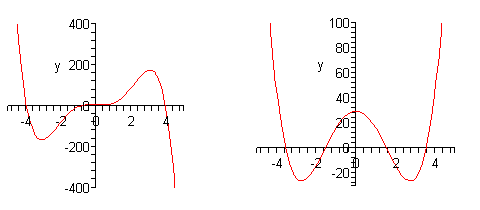
\includegraphics[width=0.75\textwidth]{imgs/image001.png}
    \end{figure}


\subsection{Symmetry in Polynomial Functions}
A polynomial function is called an even function if the exponent of each term of the equation is even. The value of the function would be the same if you subbed in a positive value or its opposite negative value.
$$f(x) = f(-x)$$ Because of this, the function will be symmetric about the y-axis

A polynomial function is called an odd function if the exponent of each term of the equation is odd. The value of the function would have the opposite sign if you
subbed in a positive value of its opposite negative value
$$f(-x) = -f(x)$$
Because of this, the function will be symmetric about the origin. 
\subsection{Transformations of Power Functions}
\begin{itemize}
    \item \textbf{Vertical Shift:} Value of $C$ in $f(x) = a[k(x - d)]^n + c$
    \begin{itemize}
        \item $C > 0$: Shift $C$ units up
        \item $C < 0$: Shift $C$ units down
    \end{itemize}
    
    \item \textbf{Horizontal Shift:} Value of $h$ in $f(x) = a[k(x - d)]^n + c$
    \begin{itemize}
        \item $d > 0$: Shift $|d|$ units right
        \item $d < 0$: Shift $|d|$ units left
    \end{itemize}
    
    \item \textbf{Vertical Stretch/Compression and Reflection:} Value of $a$ in $f(x) = a[k(x - d)]^n + c$
    \begin{itemize}
        \item $a > 1$ or $a < -1$: Vertical stretch by a factor of $|a|$
        \item $-1 < a < 1$: Vertical compression by a factor of $|a|$
        \item $a < 0$: Vertical reflection (reflection in the $x$-axis)
    \end{itemize}
    
    \item \textbf{Horizontal Compression/Stretch and Reflection:} Value of $k$ in $f(x) = a[k(x - d)]^n + c$
    \begin{itemize}
        \item $k > 1$ or $k < -1$: Horizontal compression by a factor of $|k|$
        \item $-1 < k < 1$: Horizontal stretch by a factor of $|k|$
        \item $k < 0$: Horizontal reflection (reflection in the $y$-axis)
    \end{itemize}
\end{itemize}

\textbf{Note:}
\begin{itemize}
    \item $C$ and $d$ cause vertical transformations and therefore affect the $y$-coordinates of the function.
    \item $a$ and $k$ cause horizontal transformations and therefore affect the $x$-coordinates of the function.
    \item When applying transformations to a parent function, make sure to apply the transformations represented by $C$ and $d$ before the transformations represented by $a$ and $k$.
    \item We can use the mapping $(x,y) \to \left( \frac{x}{k}+d, ay+c\right)$ to transform every point on the original power function into the new power function
\end{itemize}
\newpage
\subsection*{Intro To Absolute Value}
\textbf{Absolute value:} $f(x)= |x|$, the definition that "x" is from the origin on the number line. \\ 
In general:\\
$$
|f(x)|=
\begin{cases}
f(x) &, f(x) \ge 0\\
-f(x) &, f(x) < 0
\end{cases}
$$
The absolute value of a number is its distance from 0. For example, the absolute value of 4 is 4:
\begin{center}
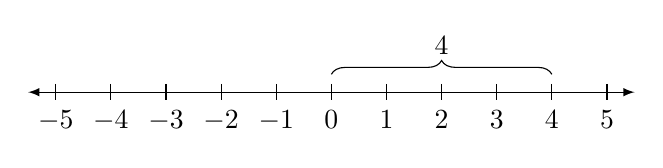
\begin{tikzpicture}[>=latex, scale=0.7]
    \draw[latex-latex] (-5.5,0) -- (5.5,0);
    \foreach \x in {-5,...,5}
    \draw (\x,0.15) -- (\x,-0.15) node[below] {$\x$};
   
    \draw[-,decorate,decoration={brace,amplitude=5pt,raise=1.5ex}]
      (0,0) -- (4,0) node[midway,above=1em]{$4$};
\end{tikzpicture}
\end{center}

This seems kind of obvious. Of course, the distance from 0 to 4 is 4. Where absolute value gets interesting is with negative numbers. \\ \\
For example, the absolute value of -4 is also 4:
\begin{center}
    
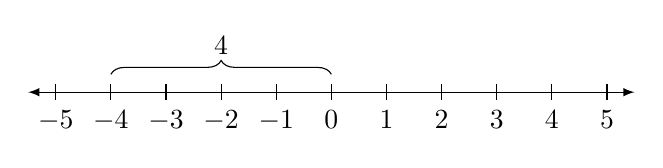
\begin{tikzpicture}[>=latex, scale=0.7]
    % Axis
    \draw[latex-latex] (-5.5,0) -- (5.5,0);
    \foreach \x in {-5,...,5}
    \draw (\x,0.15) -- (\x,-0.15) node[below] {$\x$};
   
    % Brace
    \draw[-,decorate,decoration={brace,amplitude=5pt,raise=1.5ex}]
      (-4,0) -- (0,0) node[midway,above=1em]{$4$};
\end{tikzpicture}
\end{center}

\subsection*{The absolute value symbol}
The symbol for absolute value is a bar \texttt{|} on each side of the number. \\
For example, instead of writing
"the absolute value of -6", we can just write |-6|. \\\\
\textbf{Odd functions:} A function $f(x)$ is odd if $f(-x)= -f(x)$. Symmetric about the origin or reflection along both the x and y axis. \\ 
$\quad f(x)=-2x^3+x$, is an odd function since $f(-x)=-2(-x)^3+(-x)$ \\  \\
\textbf{Note:}$$f(-x)=-f(x)$$ \\ 
For polynomial functions, the function is an odd function if all exponents are odd. \\ 
\textbf{Even functions:} A function $f(x)$ is even if $f(-x)=f(x)$. Symmetric about the y-axis. \\ 
i.e $\quad f(x)=3x^4+2x^2-2$, is an even function since function if all the exponents are even. \\ 
\newpage 
\subsection{Slopes of Secants and Average Rate of Change}
\textbf{Key Concepts}

\begin{itemize}
    \item A secant is a straight line that connects two points on a curve.
    \item Rate of Change (Slope) is a measure of how quickly one quantity (the dependent variable) changes with respect to another quantity (the independent variable).
There are two types of rates of change, average and instantaneous.
\end{itemize}



\subsubsection{Average rates of change}
    represent the rate of change over a specified interval corresponding to the slope of a secant between two points $P_1 (x_1, y_1)$ and $P_2(X_2,Y_2)$ on a curve
\begin{figure}[h]
    \centering
    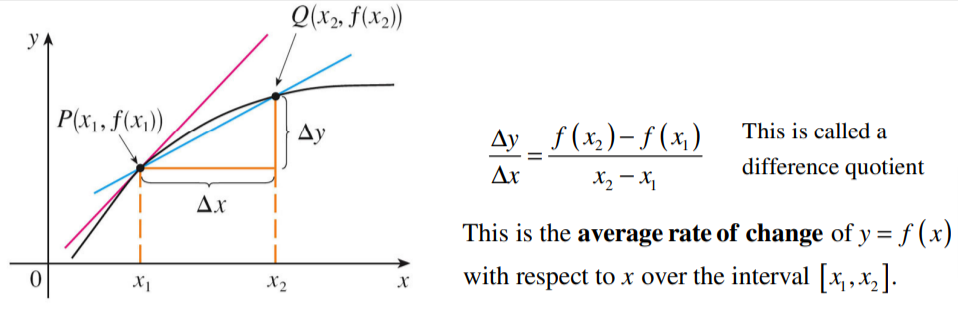
\includegraphics[width=0.9\textwidth]{imgs/Slopes of Secants and Average Rate of Change.png}
    \end{figure}
    
An average rate of change can be determined by calculating the slope between two points given in a table of values or by using an equation.

\subsection{Slopes of Tangents and Instantaneous Rate of Change}
\begin{enumerate}
    \item A tangent to a curve is a line that intersects a curve at exactly one point.
    \item An instantaneous rate of change corresponds to the slope of a tangent at a point on a curve.
    \item An approximate value for an instantaneous rate of change at a point may be determined using....
\end{enumerate}
\begin{itemize}
\item a graph, either by estimating the slope of a secant passing through that point OR by sketching the tangent and estimating the slope between the tangent point and a second point on the approximate tangent line.
\item a table of values, by estimating the slope between the point and a nearby point in the table.
\item an equation, by estimating the slope using a very short interval between the tangent point and a second point found using the equation.
\end{itemize}
\subsubsection{Relationship Between the Slope of Secants and the Slope of a Tangent}
\begin{itemize}
    \item As a point Q becomes very close to a tangent point P, the slope of the secant line becomes closer to (approaches) the slope of the tangent line.
    \item Often an arrow is used to denote the word "approaches". So, the above statement may be written as follows:
    \item As Q$\to$ P, the slope of the secant PQ the slope of the tangent at P.
    \item Thus, the average rate of change between P and Q becomes closer to the value of the instantaneous rate of change at P.
\end{itemize}
\begin{figure}[h]
    \centering
    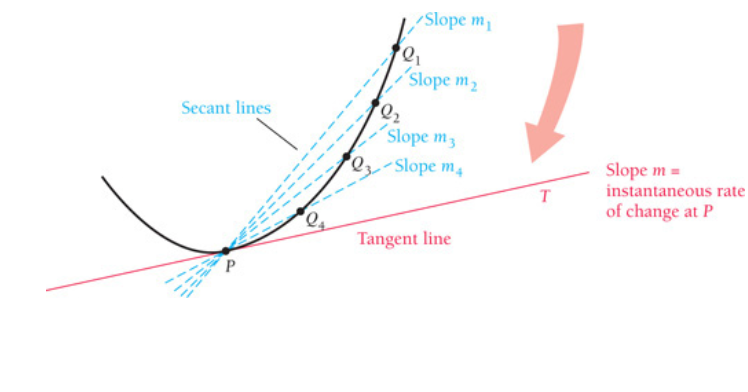
\includegraphics[width=1\textwidth]{imgs/l5olF.png}
    \end{figure}

  When $x=0, f(0)=0$, and when $x=3, f(3)=9$. The slope of the secant from $(0,0)$ to $(3,9)$ is
$$
\begin{aligned}
\frac{\Delta f(x)}{\Delta x} & =\frac{9-0}{3-0} \\
& =3
\end{aligned}
$$

When $x=1, f(1)=1$. The slope from $(1,1)$ to $(3,9)$ is
$$
\begin{aligned}
\frac{\Delta f(x)}{\Delta x} & =\frac{9-1}{3-1} \\
& =4
\end{aligned}
$$

When $x=2, f(2)=4$. The slope from $(2,4)$ to $(3,9)$ is
$$
\begin{aligned}
\frac{\Delta f(x)}{\Delta x} & =\frac{9-4}{3-2} \\
& =5
\end{aligned}
$$  
\end{document}
